% !TeX program = xelatex
\section{React Implementation}

\subsection{Grundlagen der UI}
\label{sec:reactUI}
Ein zentrales Konzept von React ist die Verwendung von Komponenten. Diese Komponenten sind wiederverwendbare UI-Elemente, die jeweils über eigenes Styling und Verhalten verfügen. 
Der wesentliche Vorteil dieses Ansatzes ist die Förderung von Wiederverwendbarkeit und Konsistenz innerhalb der Applikation. Durch die Wiederverwendung von Komponenten wird eine einheitliche Benutzeroberfläche 
gewährleistet. UI-Elemente verhalten sich in der gesamten Anwendung konsistent. Ein kohärentes Design verbessert die Benutzererfahrung und erfüllt damit zwangsläufig einen der in Sektion \ref{cha:Anforderungsanalyse:Usability} 
vorgestellten Punkte der ISO 9241-110. Zudem fördert dieser Ansatz die Entwicklungseffizienz und hält die Codebasis überschaubar.

\subsection{Grundideen des UI-Designs}
Im Gegensatz zur ursprünglichen Version, die in mehrere Aufgabenbereiche unterteilt war, empfiehlt sich nun die Integration einer zentralen Navigationsleiste für eine bessere Übersichtlichkeit. Diese ermöglicht es den Nutzern, 
problemlos zwischen verschiedenen Bereichen und Menüs zu wechseln, was die Anzahl der Klicks zwischen den Interaktionen reduziert. Dies minimiert nicht nur den Aufwand für den Nutzer, sondern verbessert auch die allgemeine Benutzererfahrung. 
Die im Kapitel \ref{cha:Usability_study} vorgestellte Studie dient zur Überprüfung der hier vorgestellten Konzepte.

Nach dem Login landet der Nutzer auf der Hauptseite, die eine Übersicht über alle verfügbaren Möglichkeiten bietet. Dies umfasst eine kurze Beschreibung des Ablaufs sowie Erklärungen zur Funktionsweise der gewählten Technologien. 
In der Navigationsleiste kann der Nutzer farblich hervorgehoben sehen, wo er sich befindet, und kann zu anderen Bereichen wie der Konfiguration der Modelle, der Verwaltung der Daten oder dem Erstellen von \textit{Projects} navigieren. 
Die Elemente \textit{Studie} und \textit{Dokumentation} sind nur temporär und sollten in der Hauptanwendung entfernt werden. Sie dienen lediglich der Durchführung und Dokumentation der Studie.
\begin{figure}[h]
    \centering
    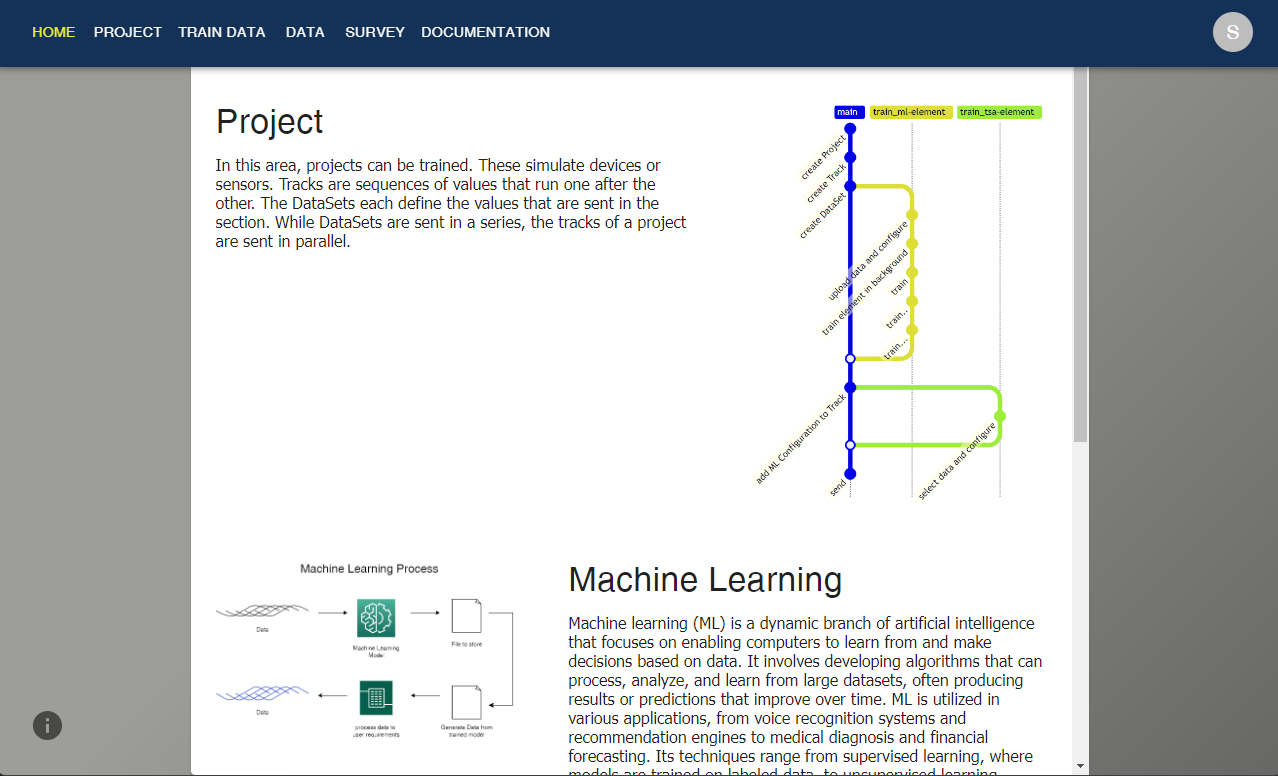
\includegraphics[width=1\linewidth]{includes/figures/new_version/main_page.png}
    \caption{vereinfachter Ablauf des Sendens von Statusinformationen mittels eines eigenen EventServices}
\label{fig:main_page}
\end{figure}





\subsection{Kommunikation mit den APIs}
\label{sec:frontendCommunication}
Um die Kommunikation und Fehlerverarbeitung zwischen den Services zu vereinheitlichen, wurde die Axios-Bibliothek integriert. 
Axios implementiert die Promise-API und ermöglicht somit asynchrones Arbeiten. Es bietet eine automatische Serialisierung von JSON zu TypeScript-Typen und Interfaces, was ein direktes, 
typenbasiertes Arbeiten mit der React-Umgebung erlaubt. Da React zudem Multi-Browser-Unterstützung bietet, kann durch die Auslagerung dieser Problematik auf eine externe Bibliothek die Webanwendung mit allen gängigen Browsern kompatibel gemacht werden.


\begin{figure}[h]
    \centering
    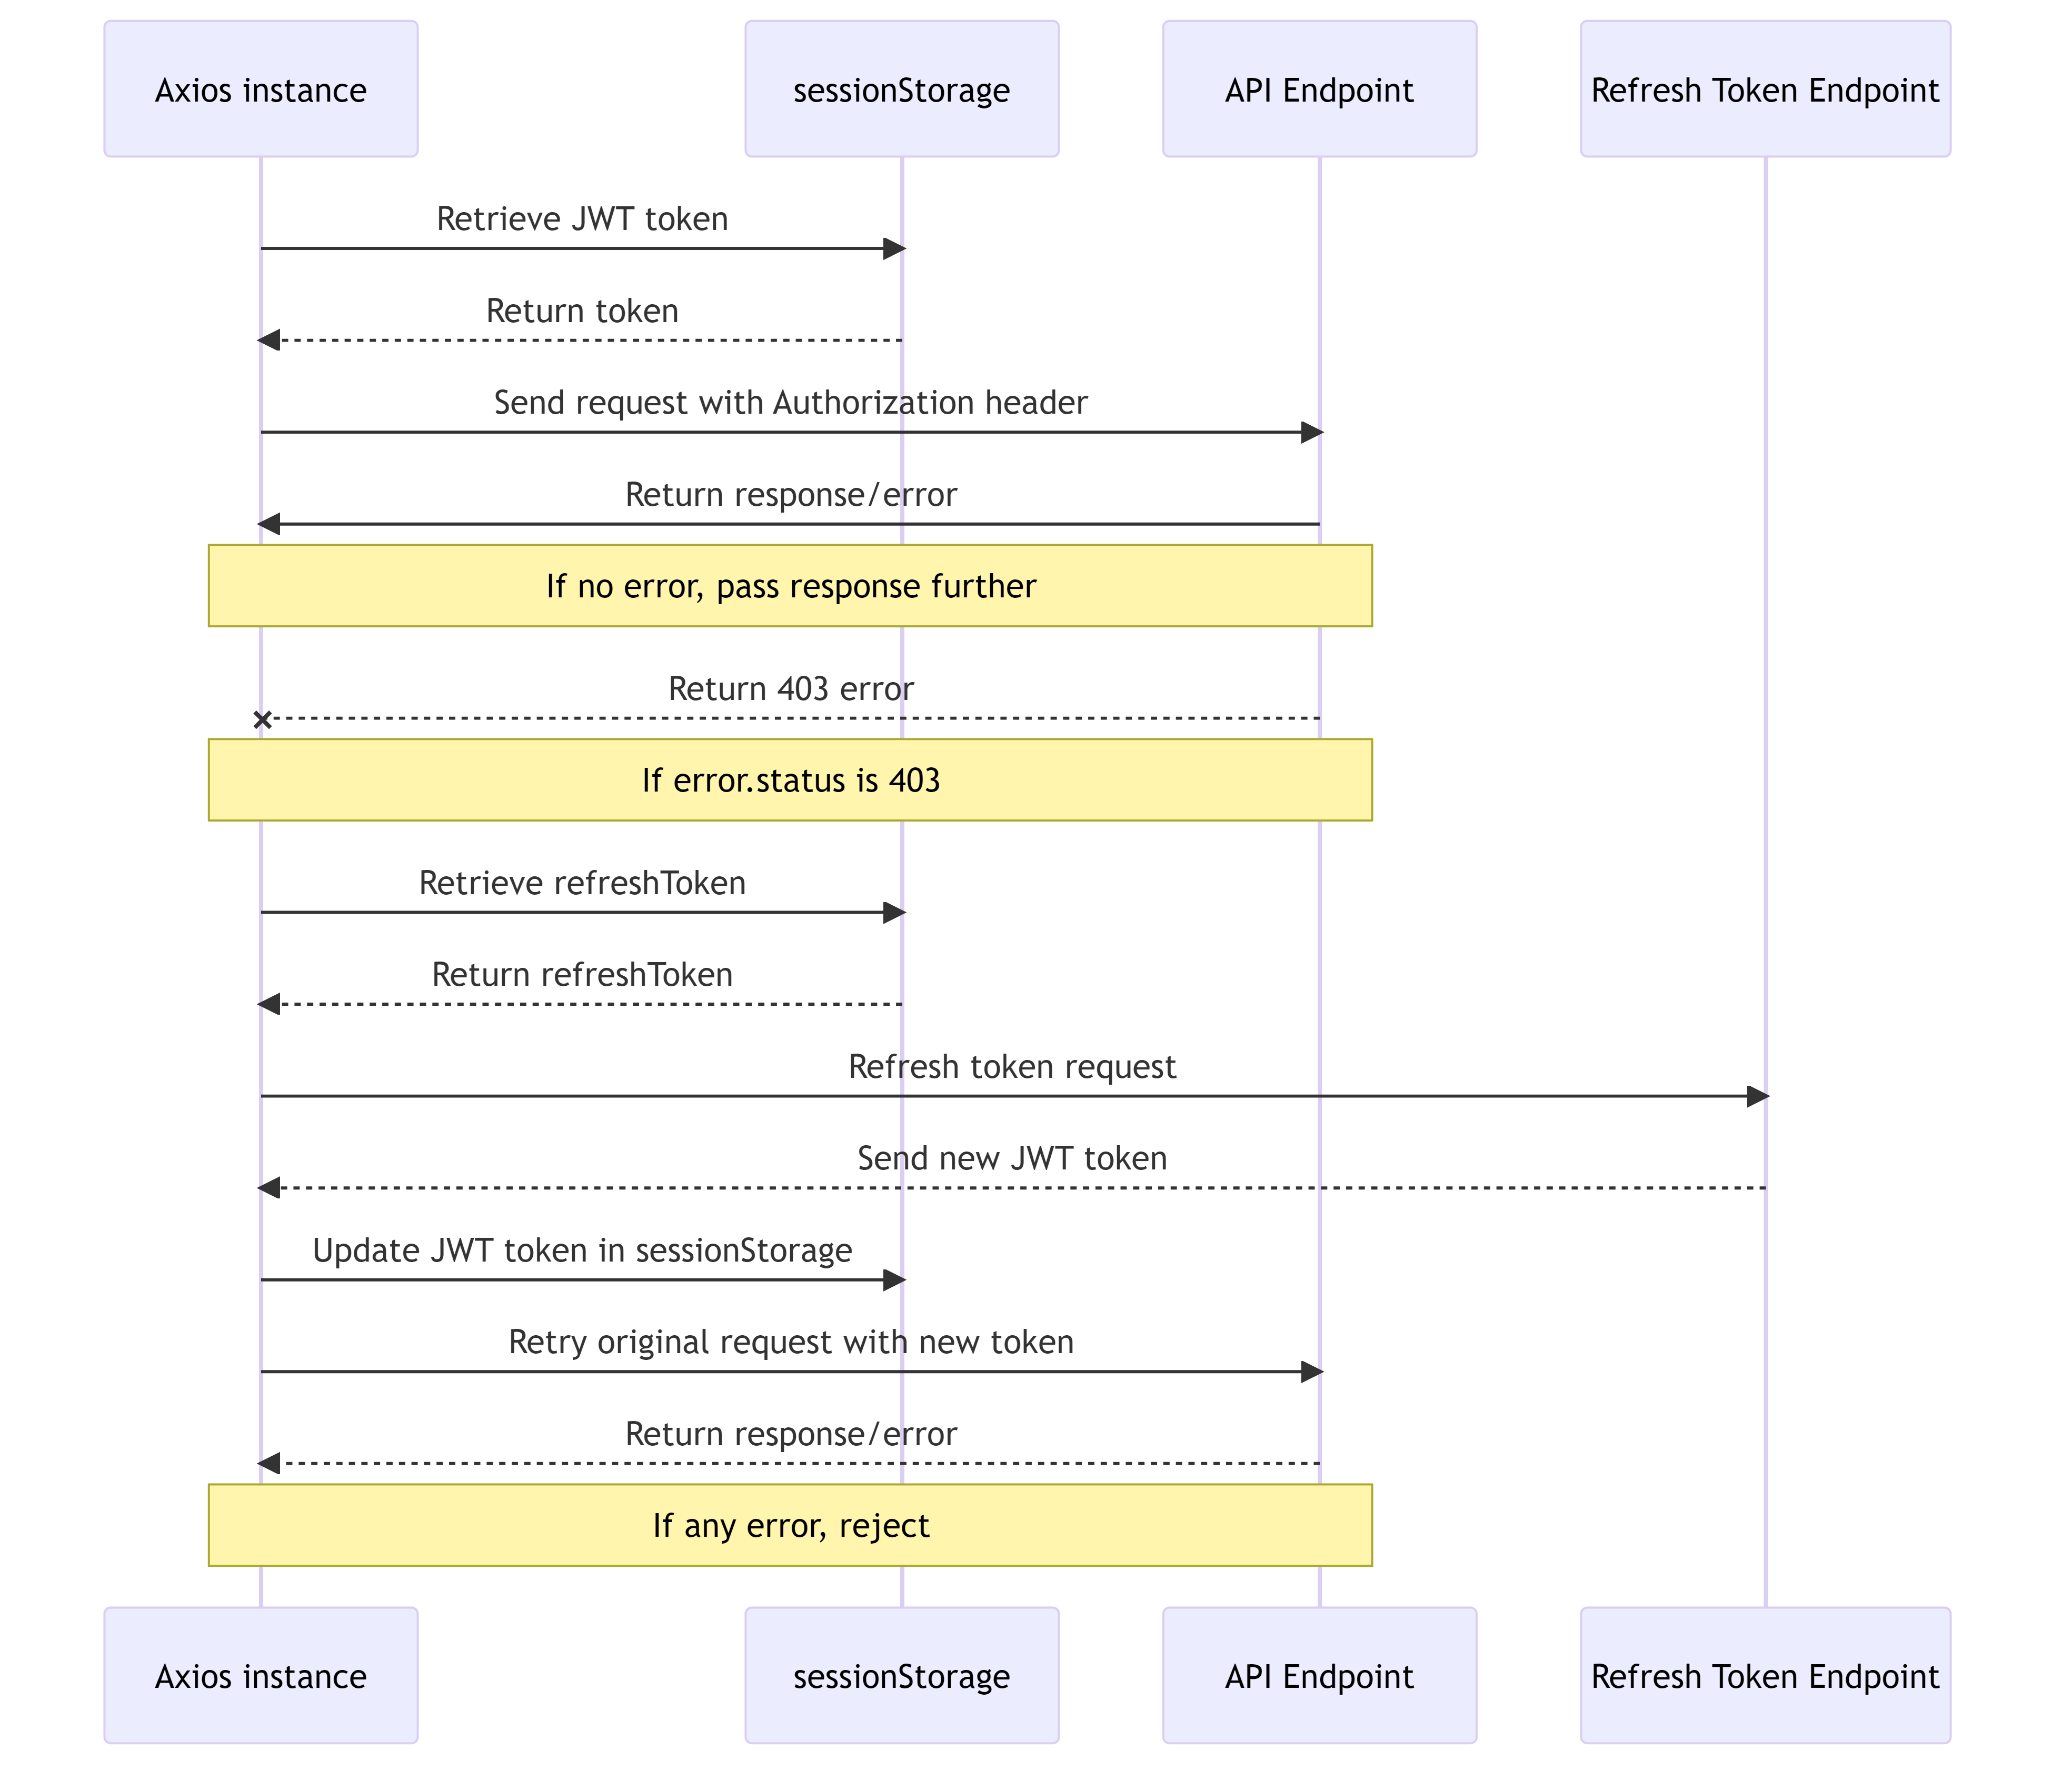
\includegraphics[width=1\linewidth]{includes/figures/axios.png}
    \caption{vereinfachter Ablauf des Sendens von Statusinformationen mittels eines eigenen EventServices}
\label{fig:react_axios}
\end{figure}

Zusätzlich erlaubt Axios die Implementierung von Interceptors. Diese überprüfen eingehende und ausgehende Requests auf ihren Status und ermöglichen eine direkte Verarbeitung. Das Konzept dahinter ist in Figur \ref{fig:react_axios} beschrieben. Fehlercodes wie '403 Not Allowed', 
die beispielsweise auftreten, wenn der JWT-Token abgelaufen ist, können durch einen separaten Refresh-Token erneuert werden, ohne dass eine erneute Anmeldung vom Nutzer erforderlich ist. Andere Fehlercodes kommen mit einem I18N-Fehlercodefeld aus dem Backend, 
um diese übersetzen zu können und so dem Nutzer genau anzuzeigen, was und warum etwas schiefgelaufen ist.


\subsection{Eingabenvalidierung über JSON Schema}
Nutzern die Eingabe möglichst einfach und verständlich zu gestalten und dabei auch Fehler zu vermeiden ist eine der wichtigsten Aufgaben eines angenehmen User Interfaces und trägt ungemein zur allgemeinen User Exerience bei.
Um dies dynamisch und flexibel zu erreichen, wurde eine Validierung der Eingaben von den ursprünglichen JsonForms durch rsjf\footnote{react-jsonschema-form ist ein react component, der ähnlich wie jsonforms, aus JSON Schemas React Components zusammenbaut} ersetzt. 
Diese überprüft die Eingaben auf ihre Korrektheit und gibt dem Nutzer ein visuelles Feedback, sollte etwas nicht stimmen. Im Gegensatz zur alten Variante aber erlaubt rsjf auch die Validierung von komplexeren Schemata und kann diese sogar in Kombination mit einer UI Definition darstellen.
Dies erlaubt es Validierung der Eingaben und Erstellung der UI zu verbinden und somit eine einheitliche und konsistente Darstellung zu gewährleisten.

 
Um die Felderbeschreibung und Fehlercodes zu übersetzen wurden Funktionen überschrieben welche das gesendete JsonSchema überschreiben und Fehlercodes sowie die dazugehörigen Argumente übersetzen. 
Dies erlaubt es dem Nutzer die Anwendung komplett in seiner eigenen Sprache zu nutzen und somit die User Experience zu verbessern.
Einen Nachteil hat dieses Vorgehen aber. Die Übersetzung der Beschreibungen setzt voraus, dass die Beschreibungen aus I18n Schlüsseln bestehen.
Fremde, oder neue User Interfaces, können die vom Backend bereitgestellten Schemata nur vernünftig darstellen, wenn diese die gleichen Schlüssel sowie Übersetzungsdateien verwenden.
Ohne eine Übersetztung ist nur der Schlüssel sichtbar, was für den Nutzer wenig hilfreich ist.

Ein weiterer großer Vorteil von rsjf ist die Möglichkeit, die Schemata dynamisch zu laden.
Anstatt wie bereits in Abschnitt \ref{sec:javaInputValidation} angedeutet die Schema fest im Code zu integrieren, was bedeutet hätte diese einzeln und für jeden Datentyp neu erstellen zu müssen, können diese durch das laden der Schema aus der API,
unabhängig vom Frontend erstellt werden und das Frontend muss lediglich eine Komponente zum laden, anzeigen und verarbeiten der Schemata bereitstellen.
Dies erleichterte besonders die Implementierung der "primitiven" Datentypen, da diese alle in der gleichen Komponente verarbeitet werden können.
Komplexere Schemata wie die der Machine Learning- und Zeit Serien Analyse Datentypen müssen aber weiterhin einzeln behandelt werden, da diese mehr Informationen benötigen als die "primitiven" Datentypen. 
Beide Datentypen verfügen über Auswahlmöglichkeiten zum genutzten Modell und dessen Konfiguration, die der Nutzer treffen muss. Diese werden in der UI als Dropdown Menüs dargestellt und in mehrere Schritte unterteilt, um die Mentale Belastung für den Nutzer möglichst gering zu halten.


\subsection{Bereitstellung von generischen Komponenten für Nutzerfeedback}
Feedback sollte konsistent sein. Egal bei welcher Aktion muss im Fehlerfall der Nutzer darüber benachtitigt werden.
MUI liefert hierfür bereits eine vorgefertigte Komponente und kann 4 verschiedene Feedbacks dem Nutzer geben.
Durch farbliche Unterscheidungen stellt es Informationen, Erfolgreiche Aktionen, Warnungen und Fehler dar. Dies natürlich in Kombination mit einer dazu passenden Erklärung.
Um diese Komponenten innerhalb der Gesammten App einzubauen wurde eine Wrapper Komponente geschrieben. 
Es erzwingt ein einheitliches Fehlerkonzept und vereinfacht die Nutzung. Da es sich um eine Austauschbare Komponente handelt, lässt sich diese später natürlich austauschen, erweitern und neuen Anforderungen anpassen.
Über die Zugabe von optionalen Übersetzungskeys ist die Fehleranzeige multilingual.
Es erlaubt damit eine einfache, dem Nutzer aus anderen Anwendungen bereits bekannte Lösung der in \ref{cha:Anforderungsanalyse:Usability} definierten Anforderung an eine Bereitstellung informativen Feedbacks.

\subsection{Bereitstellung von Mehrsprachigkeit durch i18n}
Fachsprache stellt, besonders für Nicht-Experten, eine grundlegende Herausforderung dar. Unabhängig von den Sprachkenntnissen einer Person, ist gerade die 
fachspezifische Terminologie oft schwierig zu verstehen. Nehmen wir beispielsweise Dieter Maibach, der seit vielen Jahren in einem deutschen Unternehmen arbeitet. 
Obwohl er Englisch sprechen kann, ist er nicht mit der englischen Fachsprache vertraut. Eine Software nur in einer Sprache anzubieten, die er nicht vollständig versteht, 
würde ihm erhebliche Schwierigkeiten bereiten. Eine Übersetzung der Anwendung wäre daher vorteilhaft.

Es gibt bereits zahlreiche Lösungen für dieses Problem. Im Bereich von React ist die i18next-Bibliothek weit verbreitet. Sie ermöglicht es, Anwendungen 
mithilfe von JSON-Dateien, in denen die Übersetzungen gespeichert sind, mehrsprachig zu gestalten. Der Nutzer hat dann zwei Optionen: Entweder wählt er die Sprache 
selbst aus, oder ein Detektor übernimmt die Spracheinstellung des Browsers. Eine I18N-Integration führt somit zu einer deutlich verbesserten Benutzererfahrung, da die 
Anwendung in der bevorzugten Sprache des Nutzers verwendet werden kann.

Es ist daher sinnvoll, dem Nutzer die Möglichkeit zu bieten, die Anwendung in seiner eigenen Sprache zu nutzen. Durch eine I18n-Integration kann die 
Anwendung ohne erheblichen Aufwand in verschiedene Sprachen übersetzt und somit die Benutzerfreundlichkeit erheblich gesteigert werden. Die Übersetzung der Texte 
erfolgt direkt im Frontend. Nutzer können ihre bevorzugte Sprache angeben; falls sie dies nicht tun, wird versucht, die Standardsprache des verwendeten Webbrowsers zu 
verwenden. Die Übersetzungen werden in JSON-Dateien innerhalb des Projekts gespeichert. Diese können dann über eine Komponente in die Anwendung geladen werden.

Etwas komplizierter gestaltete sich die Übersetzung der rsjf-Komponente. Da diese die Beschreibungen der Felder aus dem Schema lädt, müssen diese 
ebenfalls übersetzt werden. Ein speziell hierfür entwickelter Konverter liest das Schema aus. Anstatt mit normalen Beschreibungen zu arbeiten, mussten die 
Feldbeschreibungen als i18n-Schlüssel gespeichert werden. Dies gilt auch für die Fehlerbehandlung und -anzeige, die ebenfalls über ihre spezifischen Fehlercodes übersetzt werden müssen.
\begin{figure}[ht]
    \centering
    \begin{minipage}{0.5\textwidth}
        \centering
        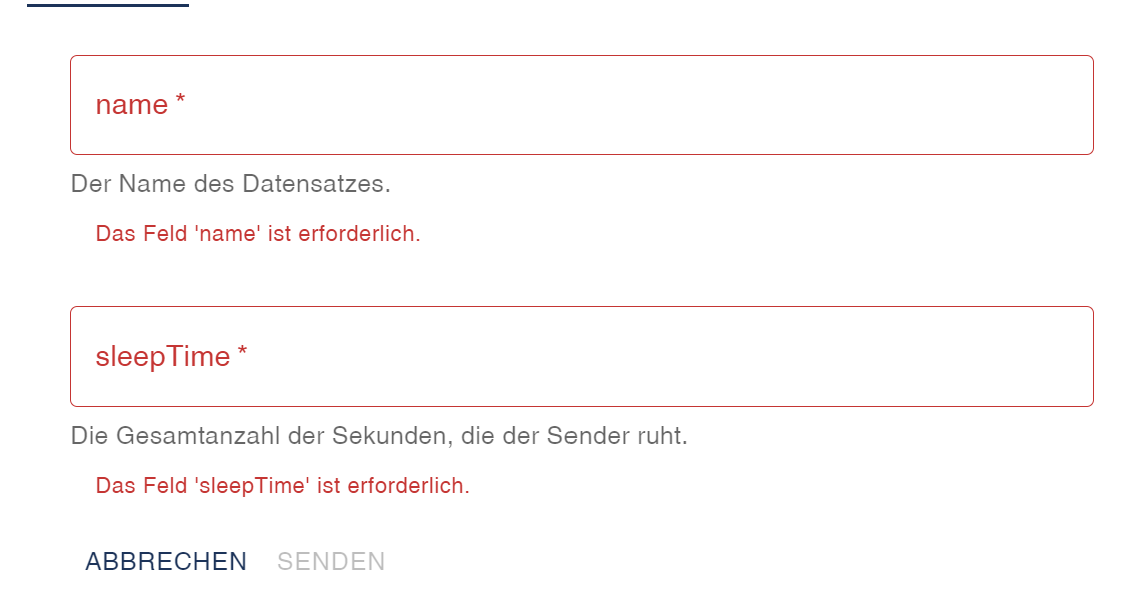
\includegraphics[width=\textwidth]{includes/figures/new_version/rsjf_translation_1.png}
        \caption{Analyse des CGAN tsgm Modells}
        \label{fig:rsjf_translation_1}
    \end{minipage}\hfill
    \begin{minipage}{0.5\textwidth}
        \centering
        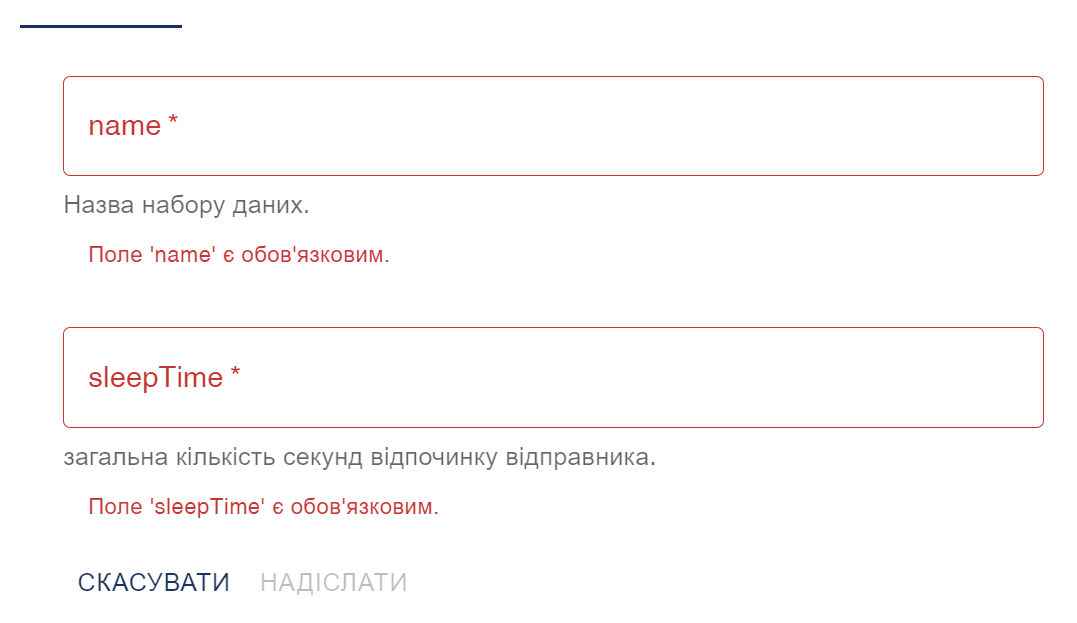
\includegraphics[width=\textwidth]{includes/figures/new_version/rsjf_translation_2.png}
        \caption{Analyse des CGAN Keras Modells}
        \label{fig:rsjf_translation_2}
    \end{minipage}
\end{figure}


\subsection{Websockets und Ihre Auswirkungen für den Nutzer}
Da, wie bereits in Spring erwähnt, es viele lang laufende Aufgaben gibt und diese für den Nutzer wenig Transparent sind, wurden in beiden APIs bereits Websocket-Endpunkte eingefügt um dem Nutzer dieses fehlende Feedback zu geben.
Diese jedoch zu implementieren stellte sich als deutlich komplexer heraus als anfangs angenommen. Security beider APIs und teilweise unterschiedlicher Protokolle, 
Zentralisierung und Verwaltung (Erstellen, auf Nachricht warten und Beenden der Verbindungen) der Websockets, das Serialisieren der Nachrichten und die multivariante Darstellung spielten hier alle mit rein.


Die Webapp muss mehrer Websockets gleichzeitig halten und verwalten können.
Nutzer können, sofern die Resourcen des Servers dies natürlich zulassen, gleichzeitig mehrere Modelle trainieren. Um es dem Nutzer hier so einfach wie möglich zu machen, hängt am Modell ein Forstschritt Element, welches numerisch und visuell den gesammten Forschritt zeigt.
Man kann aber nicht erwarten, dass der Nutzer auf der Seite des Modelles wartet, ob dieses bereits fertig trainiert ist oder noch läuft (siehe Abbildung \ref{fig:websocket_sending_projects}).
Hier kommt die zentrale Steuerung der Websockets ins Spiel. Über eine Drawer Komponente kann ein Live-Fortschritt des Modells überwacht werden. Dieses ist von jedem Punkt innerhalb der Anwendung erreichbar.
Nutzer können somit, ohne in ihrem Arbeitsfluss unterbrochen zu werden schauen, ob sie bereits neue Modelle starten können oder das trainierte Modell in ihre Tracks integrien können.
Ebendso gilt dies auch für die Projects welche gerade senden. Sollten mehrere verschiedene Projects gleichzeig senden und diese darüber hinaus auch mit zeitlich unterschiedlich langen Tracks, so kann der Nutzer dies nur schwer nachvollziehen, ohne eine Kafka Consumer implentation nebenbei laufen zu haben.
Die gleiche Drawer Komponente sorgt auch hier für klarheit, in dem sie den Fortschritt prozentual (auf die Anzahl der Tracks gerechnet) in einem Balkendiagramm anzeigzt.

\begin{figure}[h]
    \centering
    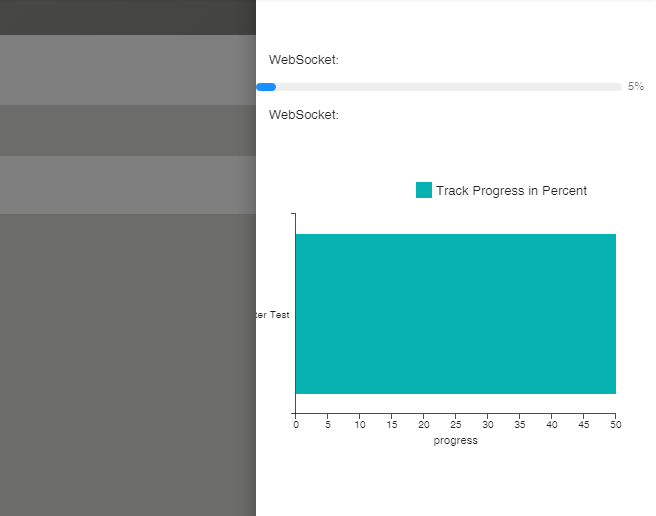
\includegraphics[width=0.9\linewidth]{includes/figures/new_version/websocket_model_training.png}
    \caption{Websocket Drawer für das Trainieren von Modellen und als Fortschrittsanzeige für sendende Projects}
\label{fig:websocket_sending_projects}
\end{figure}



\subsection{Konfiguration der Komponenten im Bereich machinelles Lernen}
Der Bereich des Machine Learnings in der Anwendung ist bewusst einfach gehalten, um eine intuitive Bedienung zu gewährleisten und Nutzer nicht mit, im Überblick unwichtigen Daten zu überlasten. Auch spiegelt dies das aktuelle \ac{API}-Design wieder, welches die Konfigurationen der Modelle über einen separaten Endpunkt verwaltet. 
Alle möglichen Konfigurationen werden beim Erstellen oder Aktualisieren des Modells vorgenommen. Diese Entscheidung basiert auf einem wichtigen Grund: 
Wie bereits in Abschnitt \ref{sec:djangoML} erörtert, stellt das Training von Modellen ein komplexes Unterfangen dar. Eine Vielzahl an Nutzereingaben kann insbesondere für fachfremde Benutzer mental anstrengend sein. 
Um den Prozess zu vereinfachen, wurde der Dialog in verschiedene, abgeschlossene Teile gegliedert. Dies reduziert die kognitive Belastung für den Benutzer. 
Im ersten Schritt gibt der Nutzer lediglich grundlegende Daten wie Namen und Beschreibung ein. Anschließend werden im nächsten Schritt die Trainingsdaten ausgewählt. Hierfür hat der Nutzer mehrere Möglichkeiten.
Wie in vielen Anwendungen bereits bekannt, gibt es eine Fläche, in die Daten über das Drag'n'Drop Prinzip abgelegt werden, alternativ wird ein Dialog zur manuellen Suchen geöffnet. 
Dann besteht noch die Möglichkeit zwischen Dateien und Elementen innerhalb der Datein zu wählen. Dieses Konzept wurde gewählt, da gerade größere CSV Dateien eine Vielzahl an Spalten enthalten können und es für den Nutzer einfacher ist, die Daten direkt in der Anwendung zu filtern, als dies in einer externen Anwendung zu tun.
Der letzte Schritt beinhaltet die spezifischen Konfigurationen für das Training des Modells. Durch ein strukturiertes und dynamisch angepasstes Eingabefeld kann der Nutzer die verschiedenen Optionen prüfen und, sofern die Daten bereits hochgeladen sind, sich einen Überblick über die Auswirkungen seiner Auswahl verschaffen. 
Der dargestellte Graph vergleicht eine originale Datei mit ihrer nach der Konfiguration bearbeiteten Version (Siehe Abbildung \ref{fig:configuration_graph_overview}) und, sofern die Zeitreihe nicht vollständig ist, zeigt auch den Unterschied der verwendeten Imputationsalgorithmen. Da dieser Prozess rechenintensiv ist, wird er nicht für alle Zeitreihen angeboten und ist nur im Dialog zu finden.

\begin{figure}[h]
    \centering
    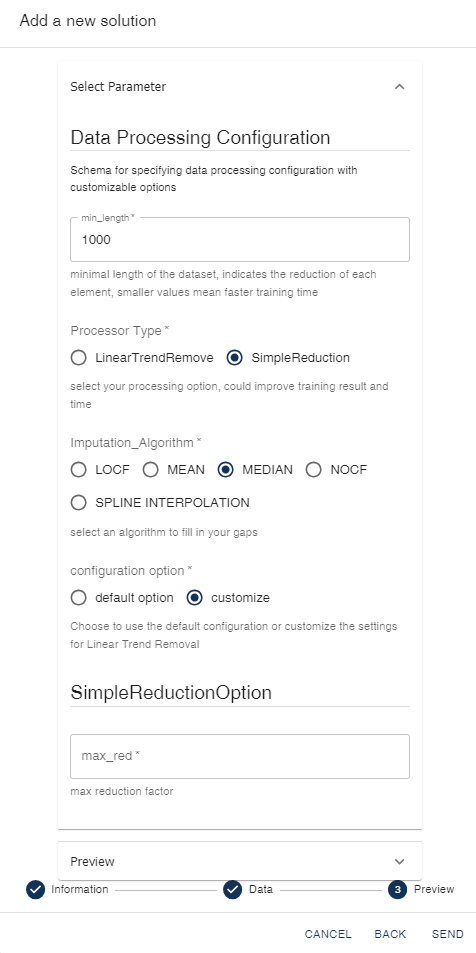
\includegraphics[width=0.5\textheight]{includes/figures/new_version/data_processing.png}
    \caption{Eingeabefeld für die Datenvorverarbeitung sowohl für die Zeit Serien Analyse als auch für das maschinelle Lernen}
\label{fig:configuration_json_schema}
\end{figure}


\begin{figure}[ht]
    \centering
    \begin{minipage}{0.5\textwidth}
        \centering
        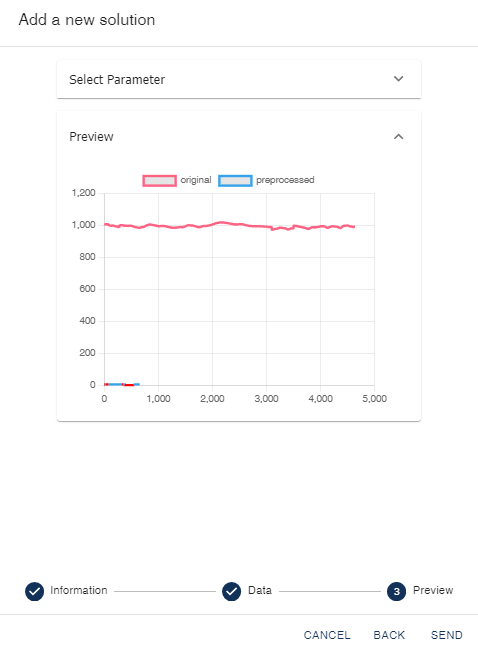
\includegraphics[width=\linewidth]{includes/figures/new_version/data_processing_2.png}
        \caption{Eingeabefeld für die Datenvorverarbeitung sowohl für die Zeit Serien Analyse als auch für das maschinelle Lernen, hier können grafisch die Unterschhiede zwischen den Originaldaten und den verarbeiteten Daten interaktive angesehen werden.}
        \label{fig:configuration_graph_overview}
    \end{minipage}\hfill
    \begin{minipage}{0.5\textwidth}
        \centering
        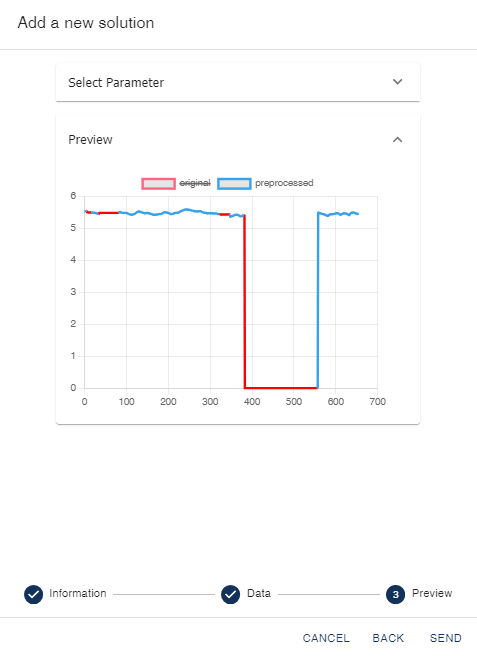
\includegraphics[width=\linewidth]{includes/figures/new_version/data_processing_3.png}
        \caption{In diesem Beispiel werden die originalen Daten ausgeblendet. Die roten Bereiche sind fehlende Werte, welche durch den Imputationsalgorithmus ersetzt wurden. Die große Lücke in der Mitte ist zu groß und wird nicht ersetzt, sondern durch ein ML Modell gefüllt.}
        \label{fig:configuration_graph_overview2}
    \end{minipage}
\end{figure}




In der Hauptansicht hat der Nutzer Zugriff auf mehrere wichtige Komponenten. Er kann seine Beschreibungen einsehen, was insbesondere bei einer Vielzahl an Modellen sehr hilfreich ist. 
Zudem bietet die Anwendung eine Übersicht, in welchen Projekten das Modell bereits eingesetzt wird, und ermöglicht einen direkten Zugriff auf diese. Weiterhin kann der Nutzer sein Modell starten und dabei einige Optionen festlegen, 
die den Trainingsverlauf wesentlich beeinflussen. Hat der Nutzer ein Modell bereits trainiert, erhält er eine Übersicht mit allen relevanten Trainingsinformationen, einschließlich Datum, Laufzeit und einem Beispielbild (Siehe Abbildung \ref{fig:ml_trained_configuration}). Dieses zeigt im direkten Vergleich die Ausgabe des Modells im Vergleich zu einem Element aus dem Trainingsdatensatz. Sollte das Ergebnis nicht den Erwartungen entsprechen, erkennt der Nutzer dies sofort und hat die Möglichkeit, das Modell mit neuen Parametern erneut zu trainieren
\begin{figure}[h]
    \centering
    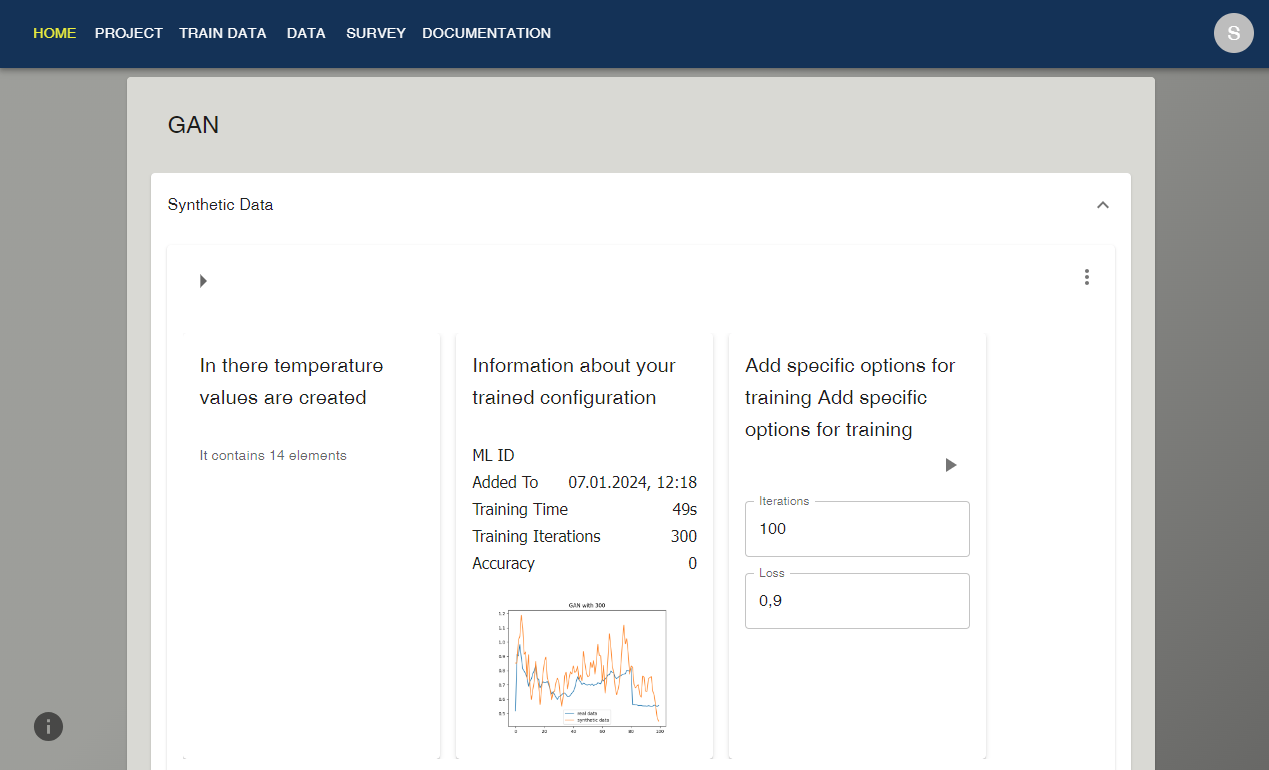
\includegraphics[width=0.9\linewidth]{includes/figures/new_version/ml_configuration.png}
    \caption{Ansicht eines trainierten Modells mit den wichtigsten Informationen und einem Beispielbild}
\label{fig:ml_trained_configuration}
\end{figure}

Zugriff auf interne Parameter der Modelle ist nicht möglich. Dies ist eine bewusste Entscheidung, um die Komplexität der Anwendung zu reduzieren und die Benutzerfreundlichkeit zu erhöhen. Es könnte durch die API angeboten werden, 
bedarf aber eines enormen Valididerungsaufwandes, da die Parameter je nach Modell stark variieren, freie Kombinationen meist nicht funktionieren und eine vernünftige \ac{API} Dokumentation hierfür enorm aufwändig wäre.

\subsection{Konfiguration der Komponenten im Bereich der Zeitreihenanalyse}
\label{sec:reactTSA}
Der Bereich der Zeitreihenanalyse ist ähnlich konzipiert wie der des Machine Learnings. Auch hier wurde Wert darauf gelegt, dieselben Komponenten zu verwenden, um den Nutzern eine konsistente und einheitliche Erfahrung zu bieten. 
Der Dialog zur Erstellung und Aktualisierung einer Konfiguration für ein Modell ist ebenfalls in mehrere Schritte unterteilt. Zunächst werden spezifische Daten für die Konfiguration eingegeben. Im zweiten Schritt erfolgt die Auswahl oder das Hochladen der Trainingsdaten. 
Im letzten Schritt kann der Nutzer die Verarbeitung der Daten anpassen, genau wie es auch in den Abbildungen \ref{fig:configuration_json_schema} und \ref{fig:configuration_graph_overview} zu sehen ist.

Ein wesentlicher Unterschied zum maschinellen Lernen besteht darin, dass die Nutzer die Modelle hier nicht trainieren müssen. Die Operationen werden direkt auf die Daten angewendet, und das Ergebnis wird dem Nutzer in verschiedenen Grafiken dargestellt. 
Bei Methoden wie der Singulärwertzerlegung (\ac{SSA}) und der empirischen Moduszerlegung (\ac{EMD}), bei denen das Signal zuerst in mehrere intrinsische Modenfunktionen (\acp{IMF}) zerlegt wird, erhält der Nutzer eine Übersicht über die einzelnen \acp{IMF}. 
Zusätzlich gibt es die Möglichkeit, diese zu verschieben, um das Ergebnis zu beeinflussen (siehe Abbildung \ref{fig:tsa_trained_configuration}). Dies kann nützlich sein, um beispielsweise Phasen zu verschieben, obwohl es kein Bestandteil der späteren Analyse ist.

Methoden wie AMIRA, die grundlegend anders funktionieren, präsentieren lediglich einen Graphen, der das Ergebnis in Arbeitsform zeigt. Dies dient dazu, die Menge der Daten, die regelmäßig zwischen der API ausgetauscht werden müssen, zu reduzieren.
\begin{figure}[h]
    \centering
    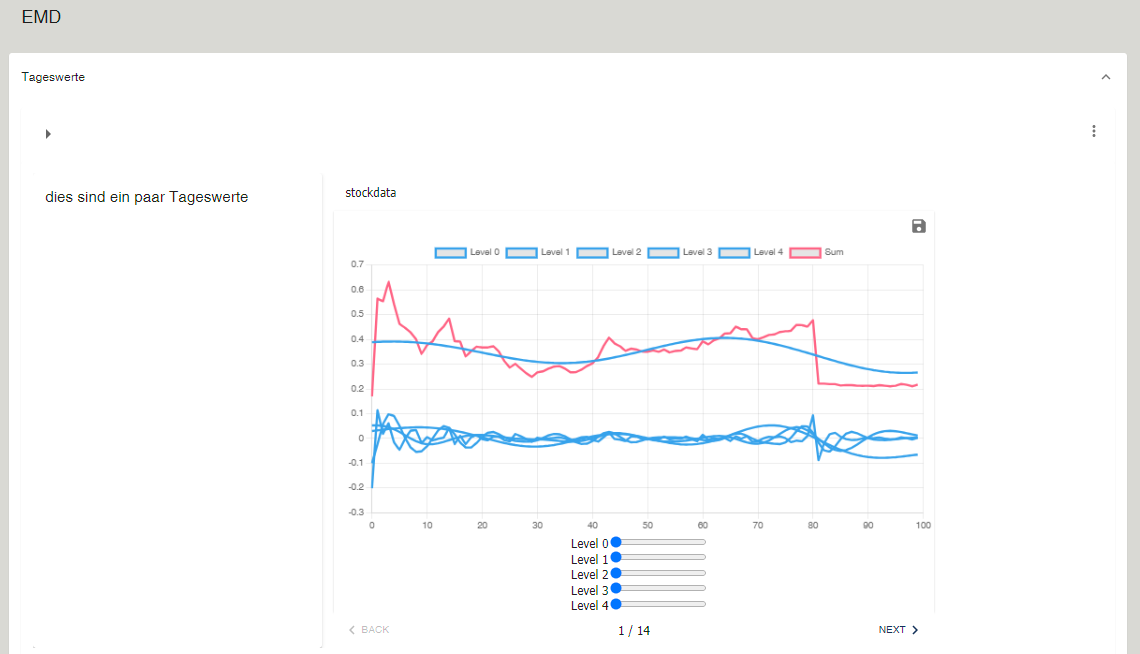
\includegraphics[width=0.9\linewidth]{includes/figures/new_version/tsa_configuration.png}
    \caption{Ansicht einer Zeitreihenzerlegung über den \ac{EMD} Algorithmus}
\label{fig:tsa_trained_configuration}
\end{figure}

Änderungen an den Modellen können nur über den Aktualisierungsdialog vorgenommen werden, indem die Konfiguration angepasst wird.
Dies ist eine bewusste Entscheidung, um die Komplexität der Anwendung zu reduzieren, da die ganzen Informationen nicht überwältigend wirken. Auch räumt es die Ansicht auf und konzentriert den Fokus auf die einzelnen Zeitreihen.
Informationen wie Laufzeit und Datum des letzten Trainings, wie es beispielsweise bei den \ac{ML} Modellen der Fall ist, ist hier nicht relevant, da die Daten in fast Echtzeit bereitgestellt werden können.

\subsection{Verwalten der hochgeladenen Daten}
Zugriff und Verwaltung der Trainingsdaten ist, wie bereits im Kaptiel \ref{cha:Anforderungsanalyse:Datenmanagement} beschrieben, ein wichtiger Bestandteil der Anwendung.
Da in den meisten Fällen Daten innerhalb der Dialoge beim Erstellen neuer Machine Learning und Time Series Analysis Konfigurationen hochgeladen werden, ist es wichtig dem Nutzer eine Möglichkeit zu bieten diese Daten auch zu verwalten.
Gerade bei komplexeren Datein, wie sie CSV Dateien mit vielen Spalten produzieren, ist ein visuelles Feedback durchaus praktisch.
Sollten Daten, oder Graphen, nicht in das gewünschte Konzept passen, kann der Nutzer diese auch direkt aus der Datei entfernen. Dies ist aber nur möglich, sofern die spezifische Datei nicht an eine Konfiguration gebunden ist.
Direkt werden dem Nutzer nur seine Datein angezeigt (Siehe Abbildung \ref{fig:data_overview_files}). Die einzelnen Graphen werden erst geladen, wenn die Datei ausgeklappt wird. Somit wird die Auslasung etwas reduziert und die Anwendung läuft flüssiger.

\begin{figure}[h]
    \centering
    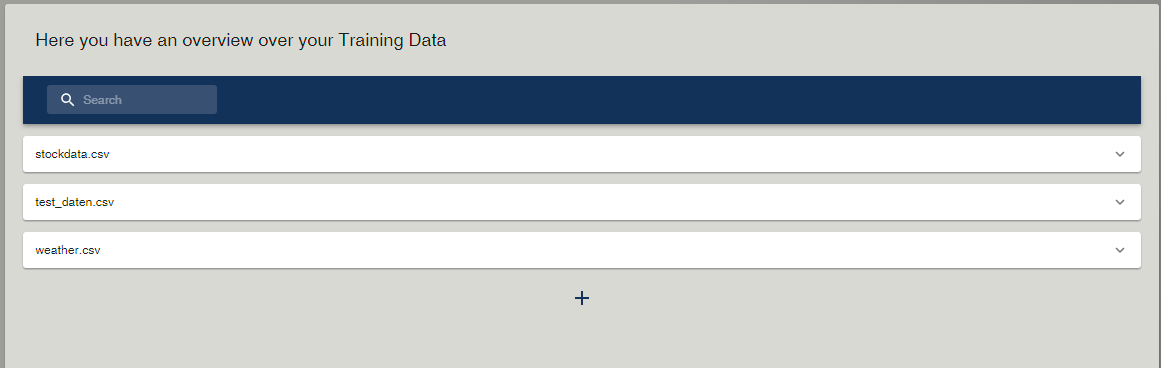
\includegraphics[width=0.9\linewidth]{includes/figures/new_version/data_overview.png}
    \caption{Übersicht über die hochgeladenen Datein und deren Inhalte}
\label{fig:data_overview_files}
\end{figure}